% !TEX root = ../report.tex
\chapter{Software Architecture}
\label{ch:software}
%IEEE Definition: A viewpoint is a collection of patterns, templates, and conventions for constructing one type of view. It defines the stakeholders whose concerns are reflected in the viewpoint and the guidelines, principles, and template models for constructing its views.
%http://www.viewpoints-and-perspectives.info/home/viewpoints/

% dijkstra quote from "Code complete p79"
The \ShortName system is a big and complex system. A developer can not, at any point in time, know the implementation of the entire system at once. "no one's skull is really big enough to contain a modern computer program" (Dijkstra 1972).\\
At any level of abstraction, the system needs to be divided into components that have the same concern. This way a developer can work on a single and comprehensible part of the system at a time. It reduces errors in the system and makes the system manageable.\\
%A view is a representation of a whole system from the perspective of a related set of concerns.[1][2]
%https://en.wikipedia.org/wiki/View_model
Each of the sections in this chapter explains a single "view" of the system, meaning it describes the system from a related set of concerns.

\section{Layer decomposition}
The layers pattern is used to create a separation of groups of classes that are reusable and share the same concerns.

\begin{figure}[H]
\centering
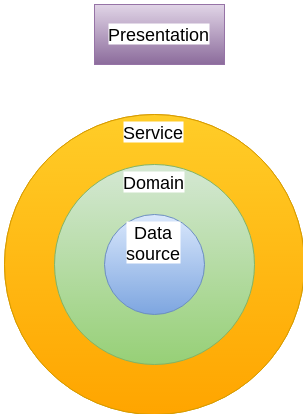
\includegraphics[scale=0.7]{7-software/images/LayersCircle.png}
\caption{Layer decomposition}
\label{fig:layerscircle}
\end{figure}

The system is decomposed into the following layers:
\begin{itemize}
\item Presentation layer
\item Service layer
\item Domain layer
\item Data source layer
\end{itemize}

\begin{description}
\item[Presentation layer] The presentation layer is concerned with presenting a graphical interface to the user (GUI). A user can use web browser and visit the \ShortName website. The browser will then show the energy statistics of that user on that browser.
%
\item[Service layer] The service layer is concerned with providing services to the clients of the system. One of these clients is the web browser of the user, as described in the presentation layer.  Figure \ref{fig:layerscircle} is drawn as a set of nested circles in order to show how the layers communicate. The domain and data source layer can not be directly contacted. In order to receive data and to get statistics, a service in the service layer has to be used.
%
\item[Domain layer] The domain layer's concern is to calculate and provide energy statistics. All the logic for generating the statistics and data that the user wants is generated in this layer
%
\item[Data source layer] The data source layer is concerned with storing and receiving data. The domain layer will use this layer for managing the data it generates. The data source layer has connections with databases and computing nodes. Computing nodes are nodes that provide data by doing computations on other data (i.e. Spark).
\end{description}


%TODO describe each layer
% The abc layer ...
% form vol4:
%%%% identify five different layers:
%%%•
%%% Presentation. This layer contains the interfaces to systems at the operation level of the automation pyramid, the so-called ‘north-bound gateways,’ as well as user-level applications that access the
%%%system’s functionality directly, such as for picking and warehouse
%%%topology management.
%%%•
%%% Business process. This layer provides the administrative and oper-
%%%ational functionality the system must support, such as stock
%%%management, order management, shipping, receiving, and material
%%%flow control.
%%%• Business objects. This layer comprises representations of domain-specific physical and logical entities on which the functionality in the business process layer operates. The main responsibility of this layer is to maintain and provide access to the warehouse topology.


The figure below shows these layers, including their responsibilities and concerns. The communication between the boxes is how the concerns are connected to each other. It is not how the actual flow of communication is handled, the communication flow will be discussed in detail later. 
%abc, add ref to communication layer thingy.

\begin{figure}[H]
\centering
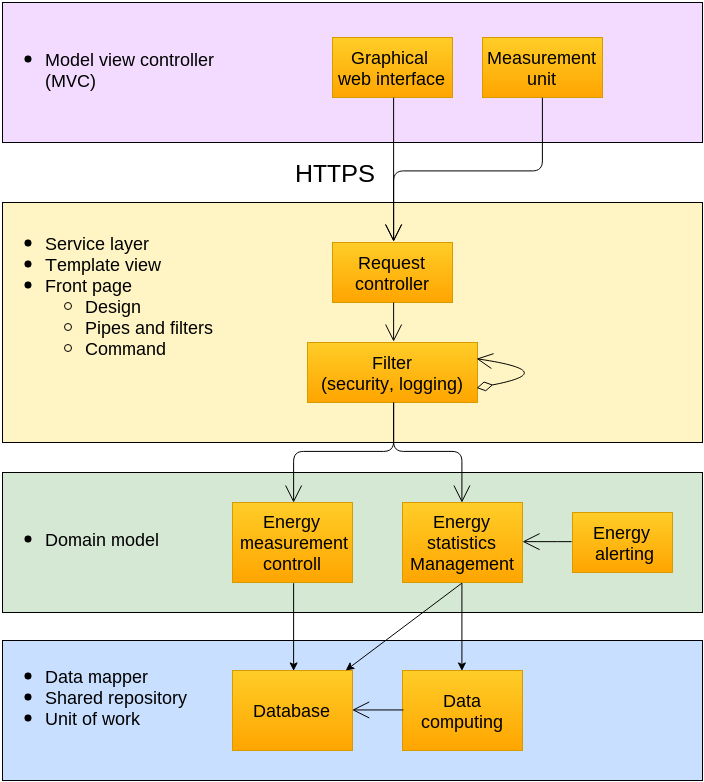
\includegraphics[scale=0.7]{7-software/images/layersflow.png}
\caption{Functionality of the system in each layer}
\label{fig:layersflow}
\end{figure}

Notice that the broker isn't mentioned. This is because the broker pattern is a pattern that handles the communication between the layers, which will be discussed in a later section.
%TODO add rprocessedeference

\section{Data flow and transformation}
\label{sec:dataflow}
This section describes how the data is handled and in the system. Requests are made to the service layer. The front page controller pattern is used to create a central set of operations to be executed for each request. These operations include logging and authenticating the request. The pipes and filters pattern to create a pipe that will execute these operations. This is shown below in figure \ref{fig:frontflow}
\begin{figure}[H]
\centering
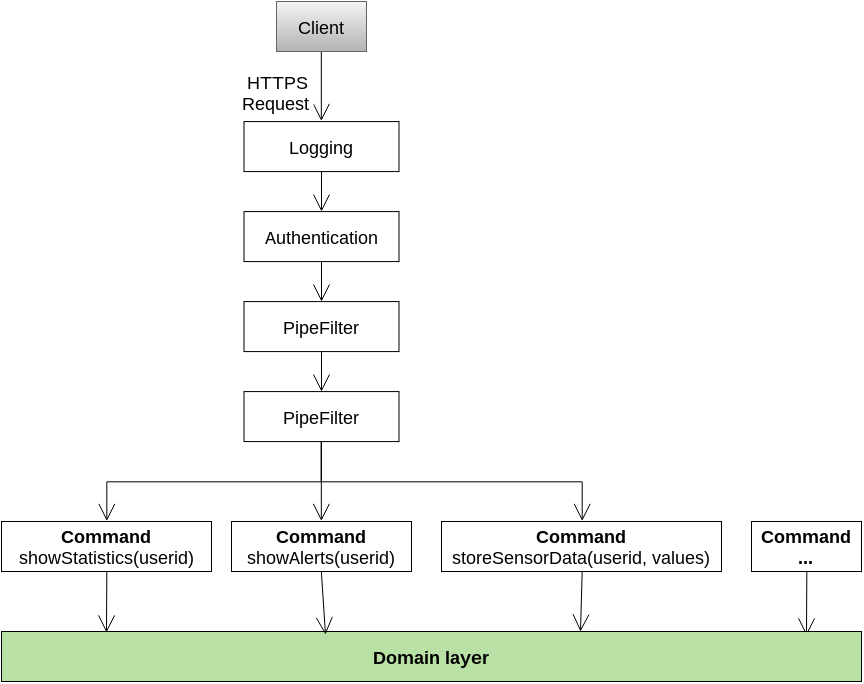
\includegraphics[width=0.8\linewidth]{7-software/images/FrontFlow.png}
\caption{Figure showing requests are piped and dispatched}
\label{fig:frontflow}
\end{figure}

The construction of the pipes will be done using the decorator pattern and the command pattern. The decorator pattern allows the system to add and remove operations to the pipe in a very flexible way. For example like $new LoggingFilter(new AuthenticationFilter(new StandardPipe()))$. It separates the operations, letting them be completely independent of each other.\\
After the request was handled by the pipe, it is dispatched to the domain layer, by using the command pattern. The command pattern is where the service layer and domain layer come together. The service layer decides what command it should execute, but the implementation of that command resides in the domain layer. The command defines an abstract "Command" class that defines a single function which is used by the service layer.\\
The domain layer then executes this command, which will do all the operations the command was created for. The image below shows a class diagram of how this information flow.

\begin{figure}[H]
\centering
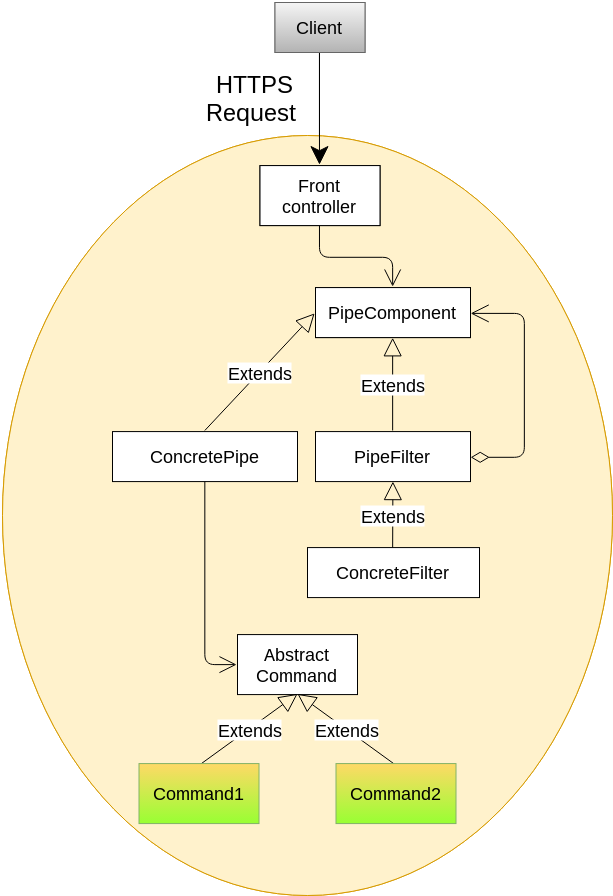
\includegraphics[width=0.8\linewidth]{7-software/images/FrontClasses.png}
\caption{Class diagram of the font page controller creating the pipes and filters}
\label{fig:frontclasses}
\end{figure}

\section{Data repository}

There are multiple components accessing a central repository of data. They do this by creating a query object and passing this to the repository. This way, the database is completely abstracted from the domain layer. The database could be replaced by a text file, without the domain layer having to change. The figure below shows an illustration of how the domain layer and the data source layer are connected.

\begin{figure}[H]
\centering
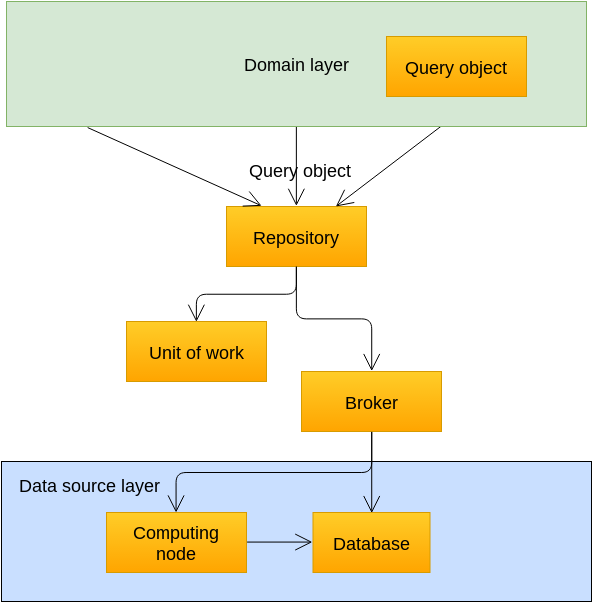
\includegraphics[width=0.8\linewidth]{7-software/images/RepoUowBroker.png}
\caption{Connection between domain layer and data source layer}
\label{fig:frontclasses}
\end{figure}

The Unit of Work pattern is used to keep track of the changes made to objects and newly created objects. Whenever an object is created, changed or deleted, the Unit of Work is told about this. 
Whenever the object can be saved to the database, the \verb|commit()| method of the Unit of Work is called, which translates the stored changes into database transactions.

A sequence diagram showing an example of this can be seen in Figure~\ref{fig:unitofworkseq}. 
This is an example of the user configuring the system. Here, the StatisticsController constructs a new Device object, which is fetched from the database and then registers itself with the Unit of Work. When the StatisticsController changes the name of this device, the device object registers itself as dirty with the Unit of Work. 
When the device object is saved, it calls \verb|commit()| on the Unit of Work, which leads to the device updating the appropriate fields in the database.

\begin{figure}[H]
\centering
\includegraphics[width=0.8\linewidth]{7-software/images/UnitOfWorkSeq.png}
\caption{Sequence diagram showing an update to a Device-object using Unit of Work}
\label{fig:unitofworkseq}
\end{figure}

The repository pattern mediates between the domain and data layer. 
The repository pattern is used by the broker pattern to get the sources the domain layer requests. The repository clients create a criteria object, specifying what kind of data is wanted. For example $criteria.equals(Device.NAME, Computer)$. Then the clients use this criteria by invoking repository.matching(criteria) to receive the data from the repository. The client just asks the data, it has no further knowledge about any interaction with any data source/data base.

\begin{figure}[H]
	\centering
	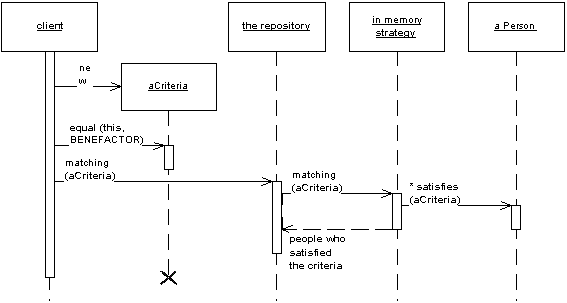
\includegraphics[width=0.8\textwidth]{7-software/images/repositorySketch.png}
	\caption{Repository View}
	\label{fig:template-view-architecture}
\end{figure}

The broker pattern is used to hide how the system interacts with the data source. Allowing the system to for example: use RPI, use a network or multiple networks, use a VPN. All without the rest of the system having to know about it.

\section{Interaction decoupling}
As mentioned in chapter \ref{ch:analysis}, MVC pattern is applied to decouple user-interface and the logic behind it. In this way, reusability is increased because the same models or controllers can be coupled with the same view. Modifiability is also increased because it becomes easier to modify a particular user interface or data model without interfering the logic, and vice-versa. Figure \ref{fig:mvc-architecture} depicts an example of MVC implementation in the HEMS.

\begin{figure}[H]
	\centering
	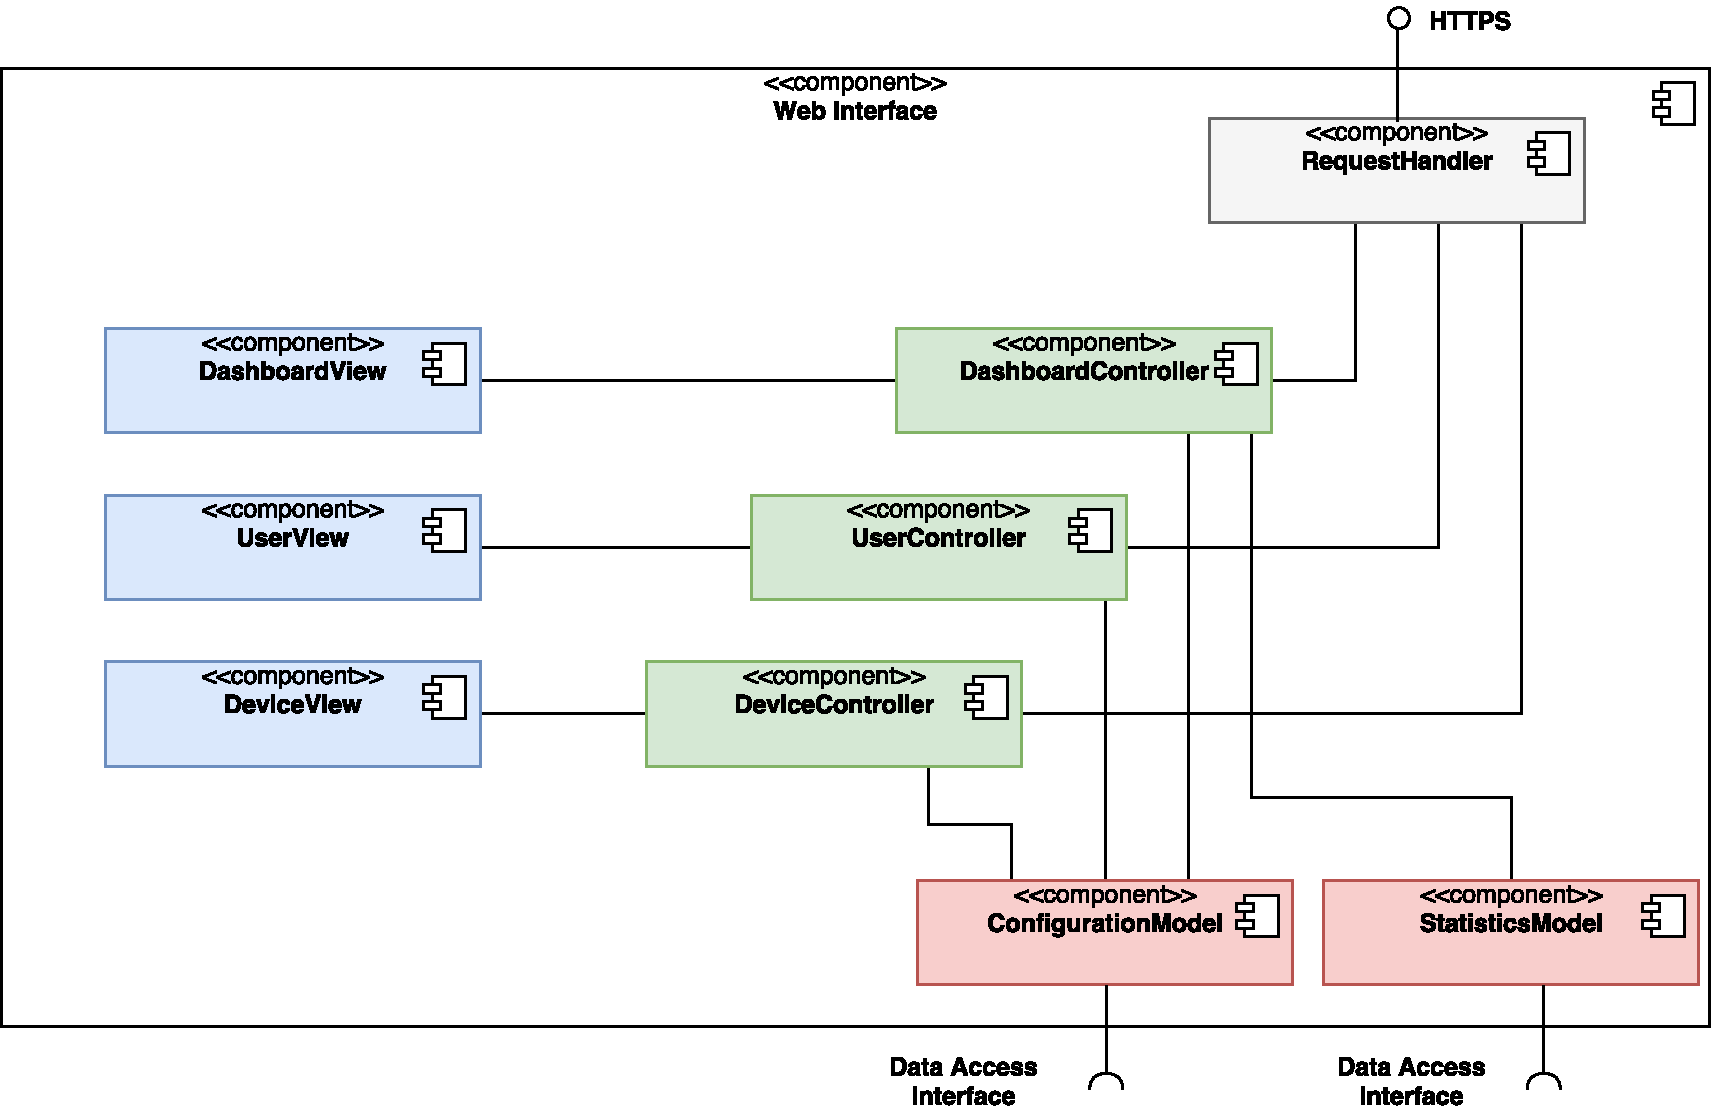
\includegraphics[width=0.8\textwidth]{7-software/images/mvc.pdf}
	\caption{Model-view-controller pattern implementation}
	\label{fig:mvc-architecture}
\end{figure}

\label{sec:template-view}
Template view is implemented in this system to make the HTML code reusable in different pages. This will also make the view structure more simple. Code duplication can be prevented because instead of duplicating the code, the HTML will use a certain template.

\begin{figure}[H]
	\centering
	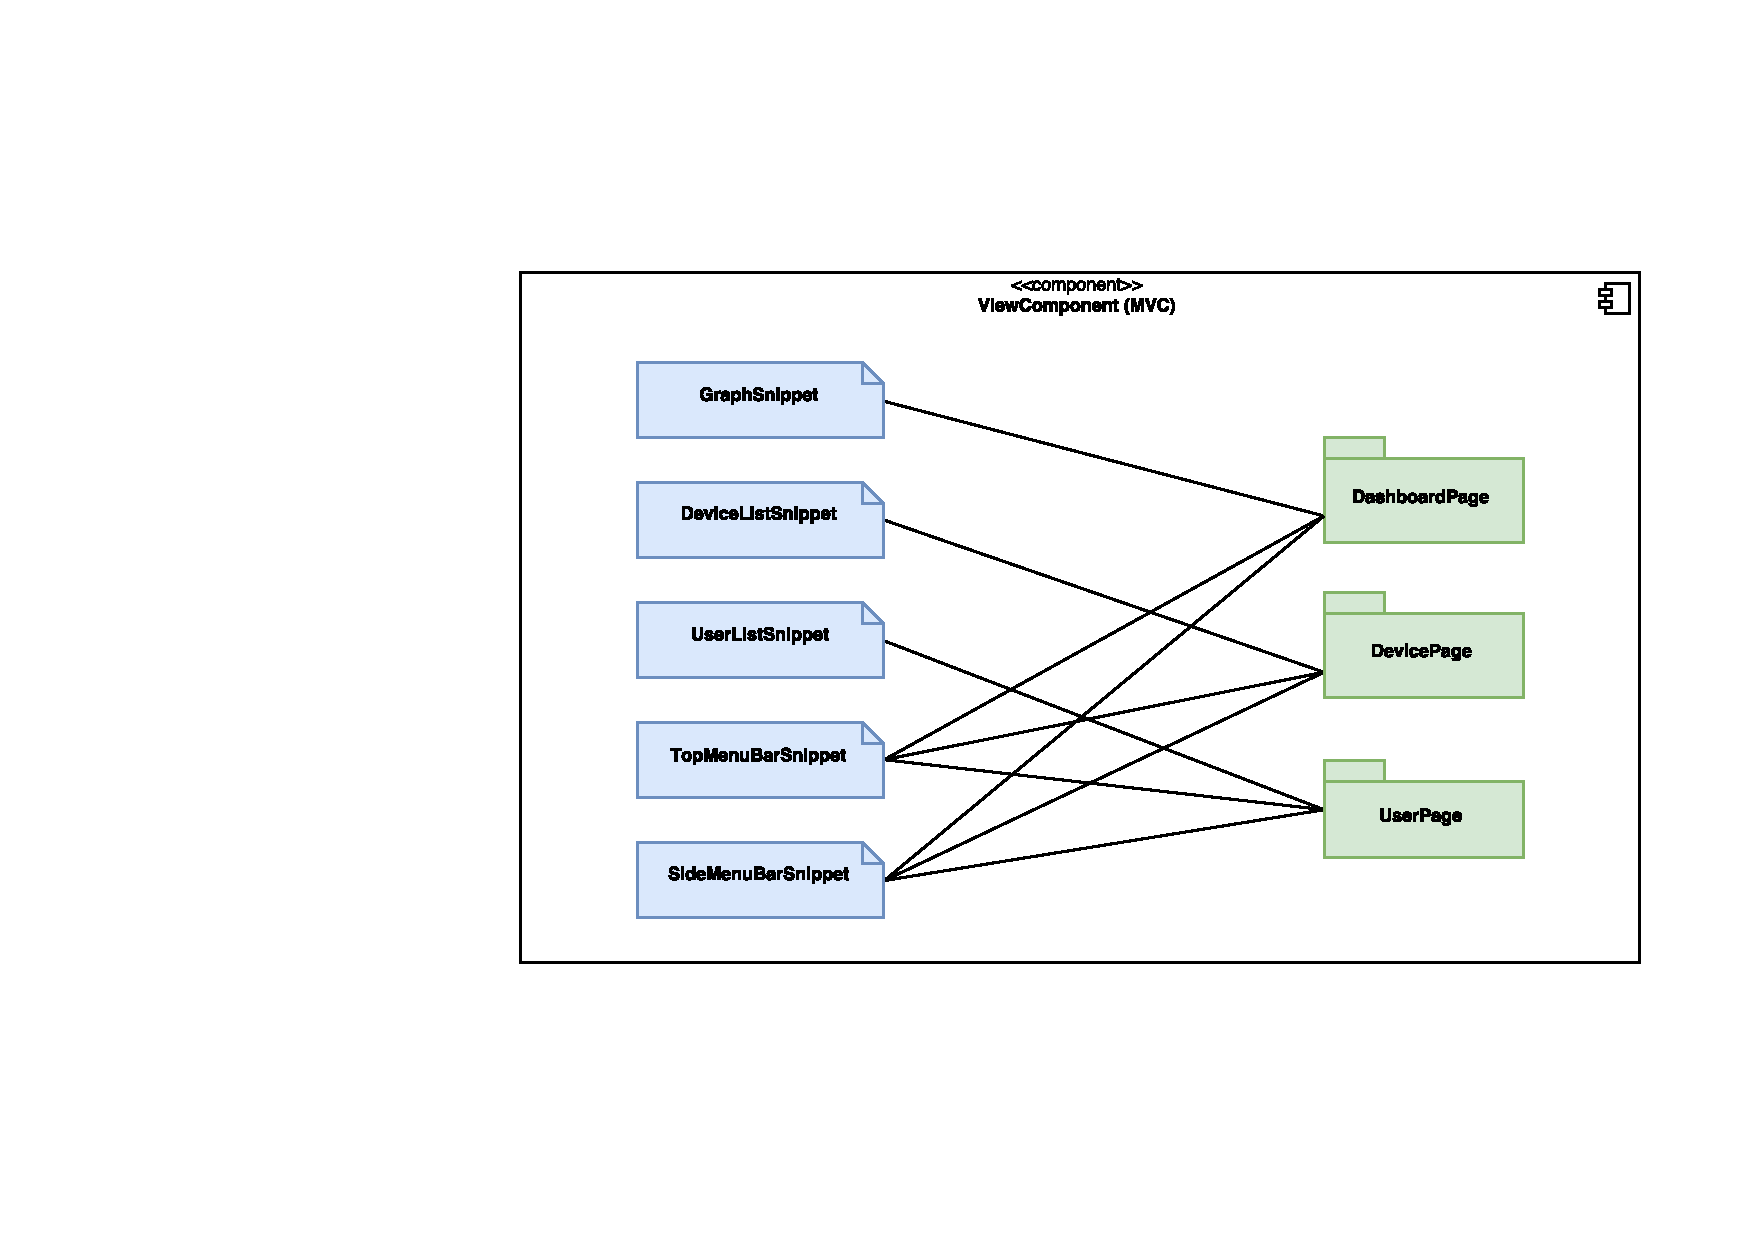
\includegraphics[width=0.7\textwidth]{7-software/images/template-view.pdf}
	\caption{Template view pattern implementation}
	\label{fig:template-view-architecture}
\end{figure}

Figure \ref{fig:template-view-architecture} shows an example of implementation of the template view pattern. Each page of the system (presented in green color) will combine several HTML code snippets (presented in blue color) together. \texttt{TopMenuBarSnippet} and \texttt{SideMenuBarSnippet} are used several times, as each page contains top menu bar and side menu bar. This is also good for expandability because the new page may just combine existing page template to create new web page.


\section{Component interaction}
This section will describe the elaborated model on the basis of the patterns used in the architecture. For each patterns, this section will describe how it is implemented and how it affects the quality attributes of the system.

\begin{figure}[H]
\centering
\includegraphics[scale=0.4]{7-software/images/Component.png}
\caption{The Layers}
\label{fig:layers}
\end{figure}
The system is divided into four layers. The first layer is the presentation layer. This layer is responsible for handling the interaction with the end user. It contains the Web Interface, which is accessible to the user over HTTPS.

The second layer is the Service Layer, see Section~\ref{sec:service-layer-pattern} for more information about this layer. This layer offers services, which can be used by other (external) components.

The third layer is the Domain Layer and is responsible for the domain logic. The Domain Model contains all the classes, has an in-memory representation of the data and contains the logic which is inherent to the objects.
It uses the Unit of Work pattern (see Section~\ref{sec:unit-of-work-pattern}) to keep track of the changes to objects, so not every change will lead to a new database call. \\
The components in the Domain Layer are connected to the Domain Model, so they have access to the classes in there. \\
The Alerting component is responsible for sending alerts by email to the end user, for which it depends on an external Email Gateway. It also uses the StatisticsService in order to compute statistics, which it needs to decide if the user should be alerted by email. \\
The Configuration and Statistics components expose their functionality to the Service Layer.
% gateway is actually also a pattern :o

The Data Source layer contains the Unit of Work, which keeps track of the changes to the objects and translates those changes to database transactions when the object is committed. The layer also contains a Database Driver, which handles the communication with the database.


%TODO Possible describe client server?....

%TODO is this needed?:
%\section{Distributed communication}
%%- Broker
%%- RPC
%%- Message queue


\section{Summary}

%TODO add the challanges.
%like on posa v4 p93
\begin{table}[H]
	\pgfplotstabletypeset[%
		KeyValue
	]{%
	key & value\\
	\textbf{Pattern} & \textbf{Challenges} \\
	\midrule
	Layers & \\
	Model-View-Controller & \\
	Template view & \\
	Service Layer & \\
	Front page & \\
	Domain model & \\
	Unit of work & \\
	Broker & \\
	Data mapper & \\
	Repository & \\
	}
\caption{UC-\arabic{uc}: Configuration- adding new devices}
\label{table:patternchallenges}
\end{table}

%% !TEX root = ../report.tex

\section{Views}
The following section will elaborate the two of the `4$+$1 model' views of the system, namely the Logic View and the Process View.

\subsection{Logic view}

\subsection{Process view}
%
%% !TEX root = ../report.tex

\clearpage
\section{Elaborated model with patterns}
This section will describe the elaborated model on the basis of the patterns used in the architecture. For each patterns, this section will describe how it is implemented and how it affects the quality attributes of the system.

\subsection{Layers pattern}
\begin{figure}[H]
\centering
\includegraphics[scale=0.4]{7-software/images/Layers.png}
\caption{The Layers}
\label{fig:layers}
\end{figure}
The system is divided into four layers. The first layer is the presentation layer. This layer is responsible for handling the interaction with the end user. It contains the Web Interface, which is accessible to the user over HTTPS.

The second layer is the Service Layer, see Section~\ref{sec:service-layer-pattern} for more information about this layer. This layer offers services, which can be used by other (external) components.

The third layer is the Domain Layer and is responsible for the domain logic. The Domain Model contains all the classes, has an in-memory representation of the data and contains the logic which is inherent to the objects.
It uses the Unit of Work pattern (see Section~\ref{sec:unit-of-work-pattern}) to keep track of the changes to objects, so not every change will lead to a new database call. \\
The components in the Domain Layer are connected to the Domain Model, so they have access to the classes in there. \\
The Alerting component is responsible for sending alerts by email to the end user, for which it depends on an external Email Gateway. It also uses the StatisticsService in order to compute statistics, which it needs to decide if the user should be alerted by email. \\
The Configuration and Statistics components expose their functionality to the Service Layer.
% gateway is actually also a pattern :o

The Data Source layer contains the Unit of Work, which keeps track of the changes to the objects and translates those changes to database transactions when the object is committed. The layer also contains a Database Driver, which handles the communication with the database.

%TODO explain individual components (in one of the views?)


\subsection{Service Layer pattern}
\label{sec:service-layer-pattern}
The service layer encapsulates the application's business logic and defines the set of available operations/interfaces to clients. In Figure~\ref{fig:layers}, the Service Layer and its components can be seen. 

It contains the `StatisticsService', which exposes an interface used by clients to store the electricity usage data and is also used by the Web Interface for computing statistics. It is also used by the Alerts component in the Domain Layer, since it needs the same computed statistics as are displayed in the web interface, to decide if the user should be alerted by email.

The Service Layer also has the `Configuration Service', which is used by the Web Interface to allow the user to add new devices, change their properties or to configure new alerts.

The Service Layer makes a common set of application functionality available to many kinds of clients. This promotes the interoperability and also prevents having duplicate code.

\subsection{Front page}
In the figure below, the structure of the front page pattern is shown, which uses the decorator and command pattern.
\label{sec:unit-of-work-pattern}
\begin{figure}[H]
\centering
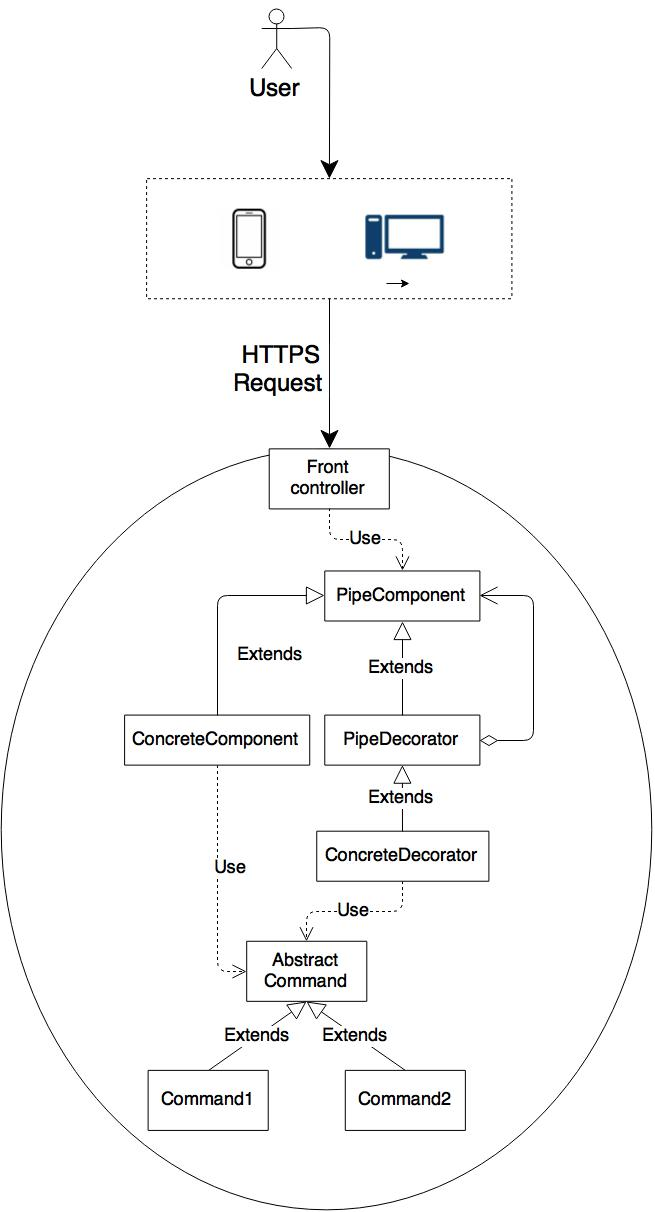
\includegraphics[scale=0.8, height=20cm]{7-software/images/frontPage.jpg}
\caption{The front controller}
\label{fig:frontcontroller}
\end{figure}

\clearpage
\subsection{Model-View-Controller}
\label{sec:mvc}
As mentioned in chapter \ref{ch:analysis}, MVC pattern is applied to decouple user-interface and the logic behind it. In this way, reusability is increased because the same models or controllers can be coupled with the same view. Modifiability is also increased because it becomes easier to modify a particular user interface or data model without interfering the logic, and vice-versa. Figure \ref{fig:mvc-architecture} depicts an example of MVC implementation in the HEMS.

\begin{figure}[H]
	\centering
	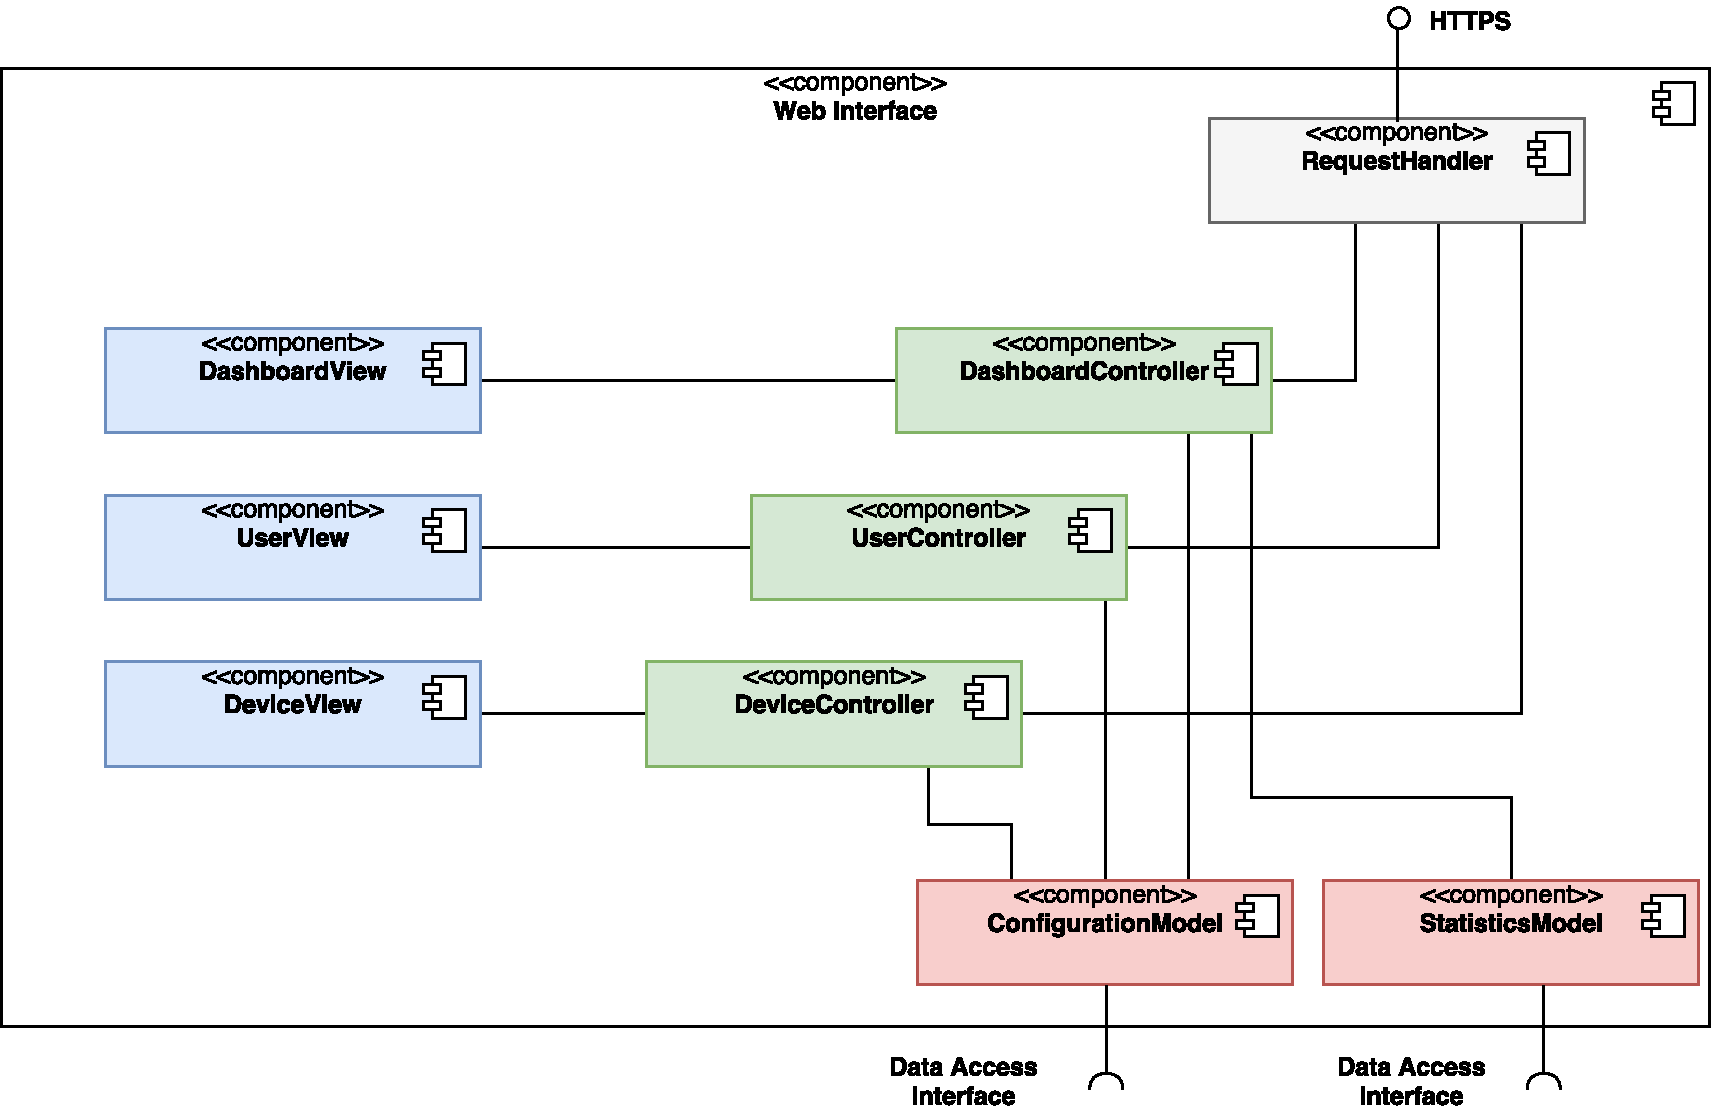
\includegraphics[width=0.8\textwidth]{7-software/images/mvc.pdf}
	\caption{Model-view-controller pattern implementation}
	\label{fig:mvc-architecture}
\end{figure}

Some models, views, and controllers are depicted in Figure \ref{fig:mvc-architecture}. Request handler handles incoming user request via HTTPS and routes it to the corresponding controller. Required data is then obtained through the models. Suitable views are used to provide user interface to the user. Some models, views, and controllers are presented in Figure \ref{fig:mvc-architecture}. However, there are more models, views, and controllers than those which are represented in the Figure \ref{fig:mvc-architecture}.

\clearpage
\subsection{Template View}
\label{sec:template-view}
Template view is implemented in this system to make the HTML code reusable in different pages. This will also make the view structure more simple. Code duplication can be prevented because instead of duplicating the code, the HTML will use a certain template.

\begin{figure}[H]
	\centering
	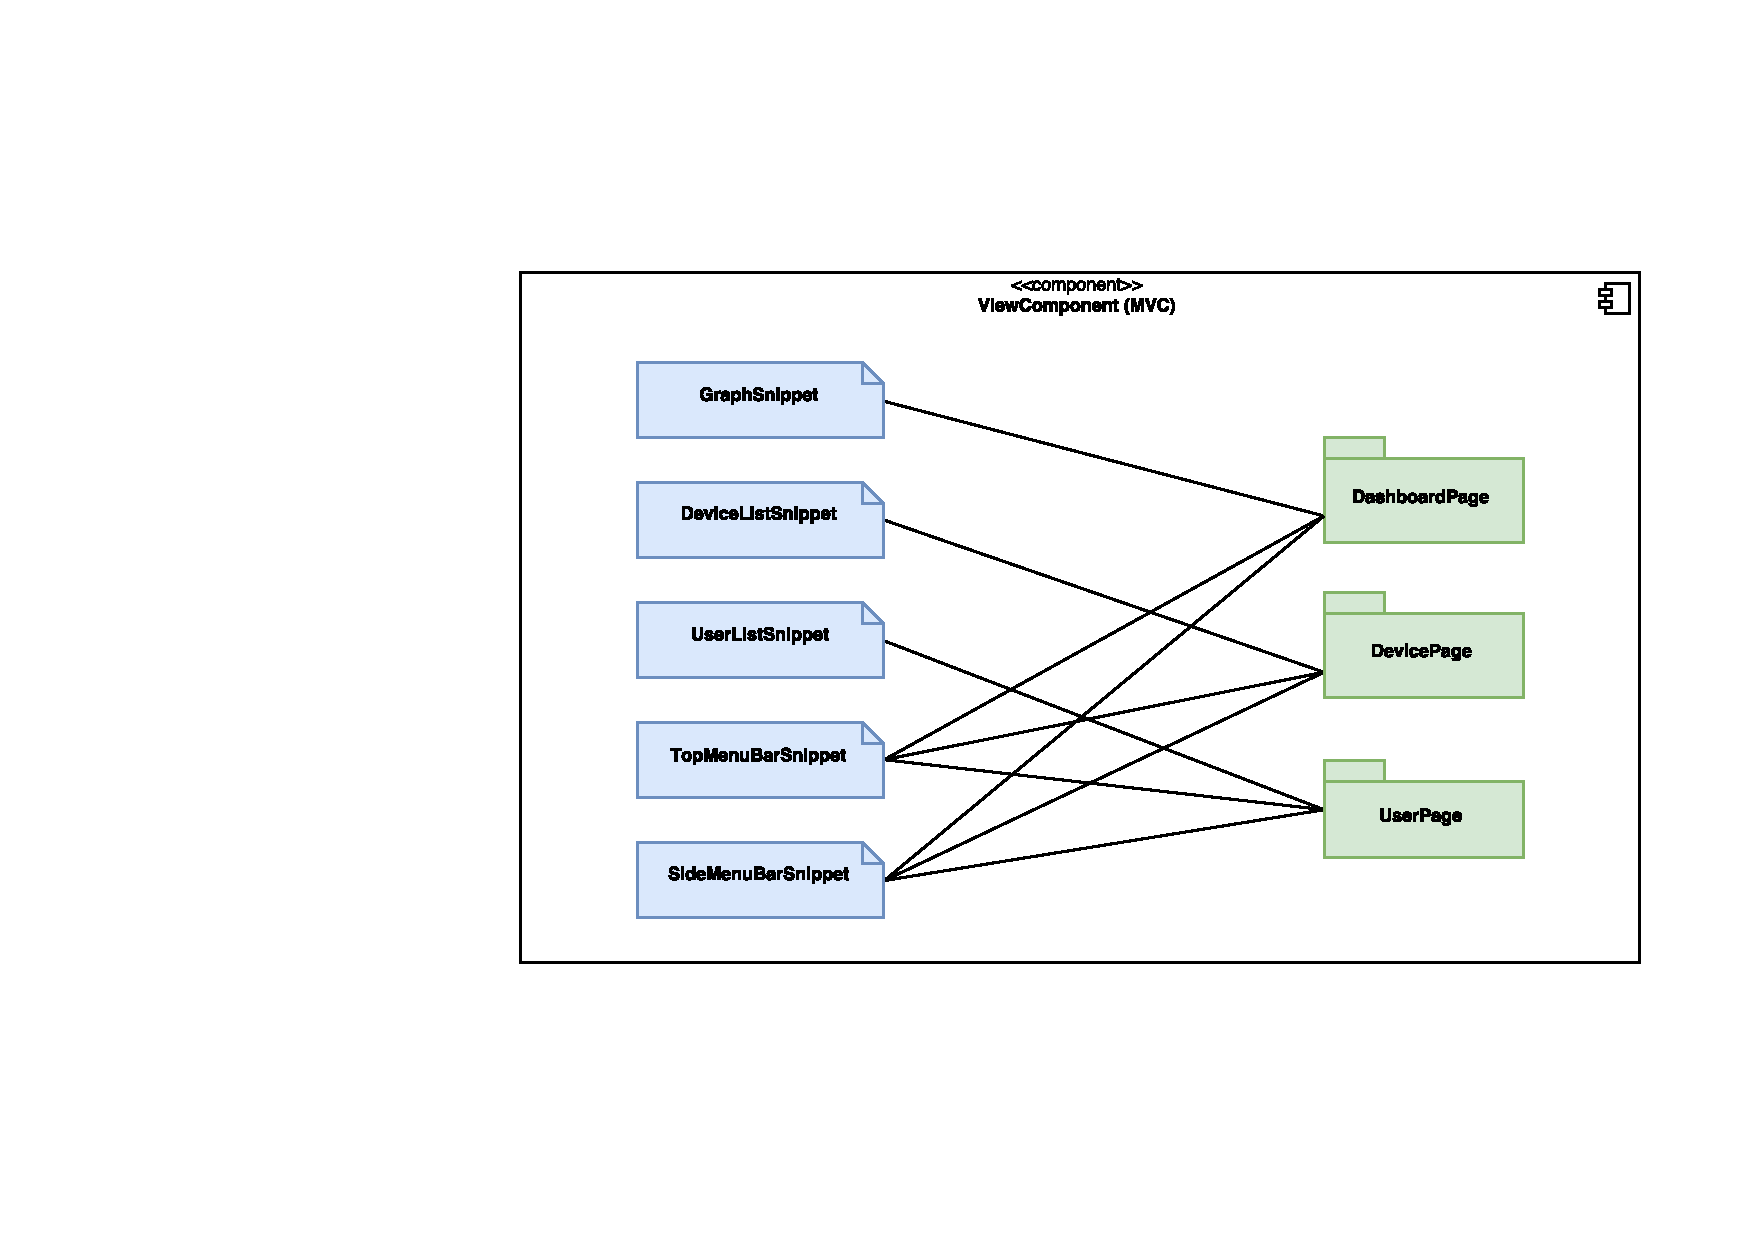
\includegraphics[width=0.7\textwidth]{7-software/images/template-view.pdf}
	\caption{Template view pattern implementation}
	\label{fig:template-view-architecture}
\end{figure}

Figure \ref{fig:template-view-architecture} shows an example of implementation of the template view pattern. Each page of the system (presented in green color) will combine several HTML code snippets (presented in blue color) together. \texttt{TopMenuBarSnippet} and \texttt{SideMenuBarSnippet} are used several times, as each page contains top menu bar and side menu bar. This is also good for expandability because the new page may just combine existing page template to create new web page.




